\section{Programming using packet transactions}
\label{s:transactions}

\begin{figure*}[!t]
\begin{minipage}{0.5\textwidth}
\begin{small}
\begin{lstlisting}[style=customc]
#define NUM_FLOWLETS    8000
#define THRESHOLD       5
#define NUM_HOPS        10

struct Packet {
  int sport;
  int dport;
  int new_hop;
  int arrival;
  int next_hop;
  int id; // array index
};

int last_time [NUM_FLOWLETS] = {0};
int saved_hop [NUM_FLOWLETS] = {0};

void flowlet(struct Packet pkt) {
  pkt.new_hop = hash3(pkt.sport,
                      pkt.dport,
                      pkt.arrival)
                % NUM_HOPS;

  pkt.id  = hash2(pkt.sport,
                  pkt.dport)
            % NUM_FLOWLETS;

  if (pkt.arrival - last_time[pkt.id] @\label{line:ifStart}@
      > THRESHOLD)
  { saved_hop[pkt.id] = pkt.new_hop; } @\label{line:ifEnd}@

  last_time[pkt.id] = pkt.arrival;
  pkt.next_hop = saved_hop[pkt.id];
}
\end{lstlisting}
\end{small}
\caption{Flowlet switching written in \pktlanguage}
\label{fig:flowlet_code}
\end{minipage}
%
\vrule\quad
%
\begin{minipage}{0.4\textwidth}
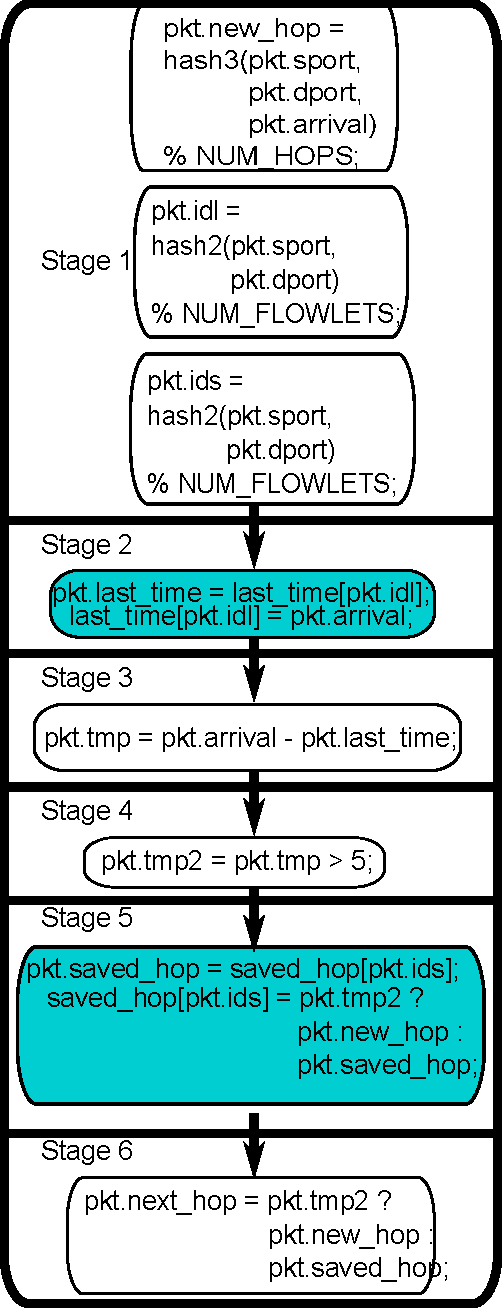
\includegraphics[width=0.8\columnwidth]{pipe.pdf}
\caption{Compiled 6-stage \absmachine pipeline implementing flowlet
switching.  Control flows from top to bottom. Atoms manipulating state are
shaded in blue.}
\label{fig:flowlet_pipeline}
\end{minipage}
\end{figure*}

We now illustrate programming using packet transactions in \pktlanguage, using
flowlet switching~\cite{flowlets} as an example. Flowlet switching is a
load-balancing algorithm that sends bursts of packets (called flowlets) from a
TCP flow on different paths, provided the bursts are separated by a large
enough interval in time to ensure packets do not arrive out of order at a TCP
receiver. Figure~\ref{fig:flowlet_code} shows flowlet switching as expressed in
\pktlanguage. For simplicity, the example hashes only the source and
destination ports; it is easy to extend it to the full 5-tuple.

This example demonstrates the core language constructs in \pktlanguage. All
packet processing happens in the context of a packet transaction (the function
\texttt{flowlet} starting at line 17). The function's argument {\tt pkt}
declares the fields in a packet (lines 5--12)\footnote{We use fields to refer
to both packet headers such as source port ({\tt sport}) and destination port
({\tt dport}) and packet metadata ({\tt id}).} that can be referenced by the
function body (lines 18--32).  In addition, the function body can reference
state variables that represent persistent state stored on the switch. These are
declared as global variables (e.g. \texttt{last\_time} and \texttt{saved\_hop}
declared on lines 14 and 15, respectively).

Conceptually, the switch invokes the packet transaction function on each
incoming packet sequentially. The function modifies the passed-in packet
argument until the end of the function body, before processing the next packet.
\pktlanguage forbids return statements, and hence execution will always end at
the end of the function body. The function may invoke \textit{intrinsics} such
as \texttt{hash2} on lines 23 and \texttt{hash3} on line 18.
Intrinsics are hardware primitives provided by the abstract machine that are
not interpreted by \pktlanguage. The \pktlanguage compiler uses an intrinsic's
signature to infer dependencies and supplies a canned run-time implementation,
but otherwise does not interpret or analyze intrinsics. The overall language is
a constrained subset of C (Table~\ref{tab:restrict}).
% Anirudh->Alvin: Yes. No one will get BNF :)
%\ac{This essentially is an imprecise version of the 
%  grammar. Maybe this is more understandable to networking audience?
\begin{table}
  \begin{tabular}{p{0.9\columnwidth}}
    No iteration (while, for, do-while).\\
    No switch, goto, return, break, or continue.\\
    No pointers.\\
    No dynamic memory allocation / heap.\\
    Array index must be constant for every execution of the transaction.\\
    No access to packet data i.e. unparsed portion of the packet.\\
    No arrays in packet fields.\\
  \end{tabular}
  \caption{Restrictions in \pktlanguage}
  \label{tab:restrict}
\end{table}

As an illustration of \pktlanguage's constraints, arrays can be used as state
variables alone but not as packet fields.  Furthermore, all accesses to a given
array within one execution of a transaction, i.e. one packet, must use the same
array index. For instance, accesses to the array \texttt{last\_time} use
the index \texttt{pkt.id}, which is constant for each packet, but changes from
one packet to the next. This restriction simplifies the treatment of arrays in
the compiler, while still allowing us to express data-plane algorithms of
practical interest. The restrictions in Table~\ref{tab:restrict} seem severe,
but are required for deterministic performance.  Memory allocation, unbounded
iteration counts, and unstructured control flow cause variable performance.
These are precisely the restrictions in \pktlanguage relative to software
routers like Click~\cite{click} with greater flexibility and variable
performance.

When compiled to a \absmachine machine (\S\ref{s:absmachine}), the \pktlanguage
compiler converts the code in Figure~\ref{fig:flowlet_code} into the atom
pipeline shown in Figure~\ref{fig:flowlet_pipeline}. The next section describes
the steps involved in this compilation.
%
%Today, programmable switch chips are
%programmed by manually specifying low-level configurations resembling
%Figure~\ref{fig:flowlet}b using a language like P4. \pktlanguage's compiler
%automates this process. \ac{I don't get this. Isn't translating from domino to 
%pisa to same as translating P4 to hardware primitives?}
% You are right. This is confusing. I am commenting this out.
% It isn't precisely correct either.
